\documentclass[a4paper,pagesize 10pt]{scrartcl}
\usepackage{graphicx}
\usepackage{scalefnt}
\usepackage{textfit}

\begin{document}


\begin{center}{\Huge\textbf{Project Proposal}}\end{center}
\begin{center}{\Large\textbf{''Head Alignment using Deep Closest Point''}}\end{center}

\section{Abstract}

% Write a short abstract / motivation of your planned project.\\\\
% Cite papers that you want to use as references (e.g. Dai et al.~\cite{dai2017shape}).\\\\
% If there is an existing implementation, specify how you would use it and what your contribution will be.
% This could be: 

With the advent of recent technologies, multi-view RGB-D acquisitions have become the prevalent way of information gathering in operating rooms (OR).
Previous works\footnote{Bachelor-Thesis written by Tony Wang last semester. If interested, it could be disclosed to the Übungsleitung :)} established the benefits of using 3D information to detect and anonymize faces in 2D images.
However, real world 3D data often suffers from noisy and incomplete point clouds, which yields in erroneous alignments using probabilistic point set alignment methods like coherent point drift (CPD)~\cite{cpd} and its variants.
In this project, we address this issue by creating and fine-tuning a deep learning based point set alignment method to achieve more robust rigid transformations on noisy and incomplete point clouds from real world data.
Our contributions are as follows:
 
\begin{itemize}
\itemsep0em
	\item We compile a new synthetic dataset consisting of different head alignment problems
	\item We show qualitative (maybe quantitative) results of the pre-trained and our fine-tuned model on data acquired from real world applications
\end{itemize}


\section{Methods}

Our goal is to align a given head mesh to the point cloud using a rigid registration. 
Previous works have used off-the-shelf methods like FilterReg~\cite{filterreg} to align the mesh to the point cloud. 
However, inadequate mesh estimations, sparse and incomplete point clouds make it unreliable in certain situations to rely on probabilistic methods.
Fig.~\ref{fig:example_mesh} depicts the upper body of a parametric human mesh model with the point cloud data.

\begin{figure}[!ht]
    \centering
    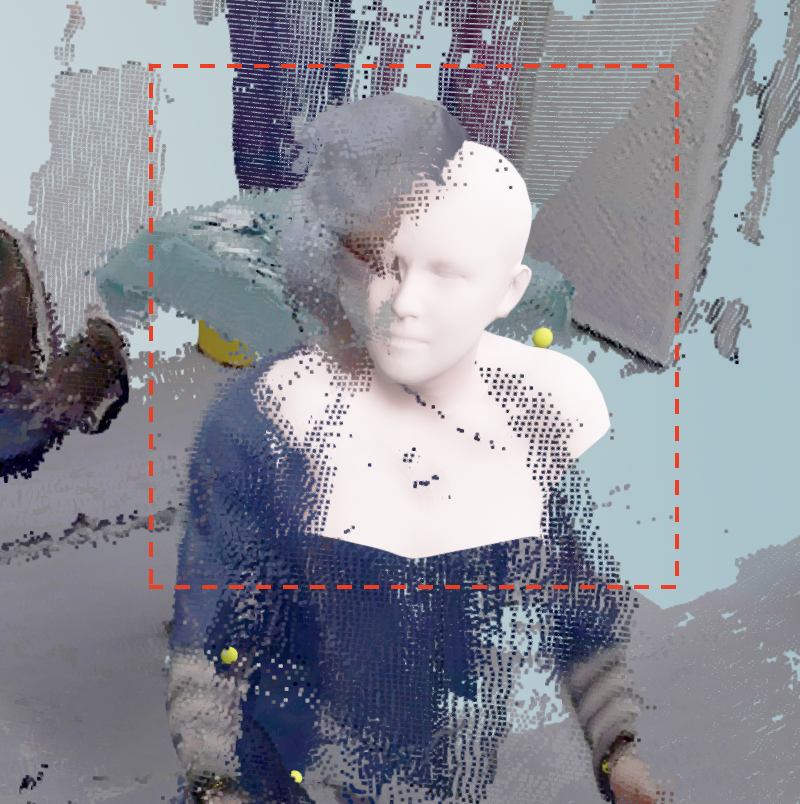
\includegraphics[width=0.95\columnwidth]{figures/issue_pointcloud.png}
    \caption{An estimated parametric human mesh model with the point cloud. For a rigid registration it would be necessary to extract the head of the mesh.}
    \label{fig:example_mesh}
\end{figure}

We use the architecture of Deep Closest Point~\cite{dcp} to train our model.
To fine-tune the model on a synthetic dataset to adapt it further to our use-case.
We generate the synthetic dataset by sampling different human poses using the parametric human mesh model SMPL~\cite{SMPL:2015} and converting it to a point cloud.
Then, we copy the head, dis-align it and apply noise on the original SMPL model point cloud.

The experiments for our evaluation will be performed on data acquired in a simulated OR from the chair of Computer Aided Medical Procedures (CAMP) at TUM (Fig.~\ref{fig:example_pcd}).
The data consists of six point clouds captured with six ceiling mounted Microsoft Azure Kinect cameras.

We could further evaluate our approach quantitatively by annotating face bounding boxes on the 2D images and reprojecting the head meshes back in 2D.

\begin{figure}[!ht]
    \centering
    \includegraphics[width=\textwidth]{figures/point_cloud.png}
    \caption{Example of a point cloud from our dataset we use for evaluation.}
    \label{fig:example_pcd}
\end{figure}

% List your requirements, e.g. dataset, which type of data you need for your approach (SDF, point clouds, etc.) and how you will generate them from the dataset you want to use.


\section{Team}
Tony Wang 03726379


% references
{\small
	\bibliographystyle{plain}
	\bibliography{bibliography}
}

\end{document}